% Options for packages loaded elsewhere
\PassOptionsToPackage{unicode}{hyperref}
\PassOptionsToPackage{hyphens}{url}
%
\documentclass[
]{article}
\usepackage{amsmath,amssymb}
\usepackage{iftex}
\ifPDFTeX
  \usepackage[T1]{fontenc}
  \usepackage[utf8]{inputenc}
  \usepackage{textcomp} % provide euro and other symbols
\else % if luatex or xetex
  \usepackage{unicode-math} % this also loads fontspec
  \defaultfontfeatures{Scale=MatchLowercase}
  \defaultfontfeatures[\rmfamily]{Ligatures=TeX,Scale=1}
\fi
\usepackage{lmodern}
\ifPDFTeX\else
  % xetex/luatex font selection
  \setmainfont[]{Times New Roman}
\fi
% Use upquote if available, for straight quotes in verbatim environments
\IfFileExists{upquote.sty}{\usepackage{upquote}}{}
\IfFileExists{microtype.sty}{% use microtype if available
  \usepackage[]{microtype}
  \UseMicrotypeSet[protrusion]{basicmath} % disable protrusion for tt fonts
}{}
\makeatletter
\@ifundefined{KOMAClassName}{% if non-KOMA class
  \IfFileExists{parskip.sty}{%
    \usepackage{parskip}
  }{% else
    \setlength{\parindent}{0pt}
    \setlength{\parskip}{6pt plus 2pt minus 1pt}}
}{% if KOMA class
  \KOMAoptions{parskip=half}}
\makeatother
\usepackage{xcolor}
\usepackage[margin=1in]{geometry}
\usepackage{graphicx}
\makeatletter
\def\maxwidth{\ifdim\Gin@nat@width>\linewidth\linewidth\else\Gin@nat@width\fi}
\def\maxheight{\ifdim\Gin@nat@height>\textheight\textheight\else\Gin@nat@height\fi}
\makeatother
% Scale images if necessary, so that they will not overflow the page
% margins by default, and it is still possible to overwrite the defaults
% using explicit options in \includegraphics[width, height, ...]{}
\setkeys{Gin}{width=\maxwidth,height=\maxheight,keepaspectratio}
% Set default figure placement to htbp
\makeatletter
\def\fps@figure{htbp}
\makeatother
\setlength{\emergencystretch}{3em} % prevent overfull lines
\providecommand{\tightlist}{%
  \setlength{\itemsep}{0pt}\setlength{\parskip}{0pt}}
\setcounter{secnumdepth}{-\maxdimen} % remove section numbering
\usepackage{booktabs}
\usepackage{longtable}
\usepackage{array}
\usepackage{multirow}
\usepackage{wrapfig}
\usepackage{float}
\usepackage{colortbl}
\usepackage{pdflscape}
\usepackage{tabu}
\usepackage{threeparttable}
\usepackage{threeparttablex}
\usepackage[normalem]{ulem}
\usepackage{makecell}
\usepackage{xcolor}
\ifLuaTeX
  \usepackage{selnolig}  % disable illegal ligatures
\fi
\IfFileExists{bookmark.sty}{\usepackage{bookmark}}{\usepackage{hyperref}}
\IfFileExists{xurl.sty}{\usepackage{xurl}}{} % add URL line breaks if available
\urlstyle{same}
\hypersetup{
  pdftitle={MUSA 5000, Homework Number 3, Logistic Regression},
  pdfauthor={Richard Barad, Dave Drennan, Jarred Randall},
  hidelinks,
  pdfcreator={LaTeX via pandoc}}

\title{MUSA 5000, Homework Number 3, Logistic Regression}
\author{Richard Barad, Dave Drennan, Jarred Randall}
\date{2023-11-28}

\begin{document}
\maketitle

{
\setcounter{tocdepth}{2}
\tableofcontents
}
\hypertarget{introduction}{%
\section{Introduction}\label{introduction}}

Driving while intoxicated and the damage that drunk drivers can cause to
individuals, families, and property is a serious issue in the United
States that results in fatalities every day - the US Department of
Transportation states that almost 30 people a day die as a result of
drunk drivers. Understanding what predictors of a crash that are
associated with drunk driving can help us better understand the nature
of these crashes and the outcomes that can occur when certain behaviors
are true in incidents that involve drunk drivers.

For this analysis, we will be using Philadelphia, PA crash data between
2008 and 2012 from the PA Department of Transportation. The data is
geocoded and was previously merged with US Census block group data to
incorporate socioeconomic features. The original data set includes
53,260 crashes and is filtered to remove nearly 10,000 crashes that
occurred in non-residential block groups to contain a total of 43,364
crashes that happened in Philadelphia residential areas.

We will conduct a logistic regression and use a combination of binary
and continuous variables, with binary variables represented by a 1 for
``Yes'' and 0 for ``No''. Throughout this report, we will also refer to
our logistic model as a logit model. Our dependent variable is
DRINKING\_D, which indicates if the driver was drunk or not, and we use
this binary variable in our logistic regression to regress it on the
following predictors:

\begin{itemize}
\item
  FATAL\_OR\_M: whether the crash resulted in a fatality or major
  injury. We speculate this may correlate with drunk driving due to the
  many deaths that are reported to occur as a result of driving while
  intoxicated.
\item
  OVERTURNED: whether the crash involved an overturned vehicle, which we
  speculate as a more serious crash incident that is more likely if the
  driver is drunk.
\item
  CELL\_PHONE: whether the crash involved a driver using a cell phone,
  which we speculate would be associated with drunk drivers since they
  are more likely to be careless behind the wheel and misjudge their
  ability to multitask effectively.
\item
  SPEEDING: whether the crash involved speeding, which we speculate
  would be associated with drunk drivers due to reckless or uninhibited
  behaviors that are often associated with being drunk.
\item
  AGGRESSIVE: whether the crash involved aggressive driving, which we
  speculate would be associated with drunk drivers for the same reasons
  as SPEEDING.
\item
  DRIVER1617: whether the crash involved a driver who is 16 or 17 years
  old, which we speculate would be associated with drunk drivers due to
  limited experience or low tolerance for alcohol, as well as the
  reasons associated with SPEEDING and AGGRESSIVE.
\item
  DRIVER65PLUS: whether the crash involved a driver who is 65+ years
  old, which we speculate would be associated with drunk drivers due to
  low tolerance for alcohol, as well as the reasons associated with
  SPEEDING and AGGRESSIVE.
\item
  PCTBACHMOR: percent of individuals 25+ years old in a block group who
  have at least a bachelor's degrees in the block group where the crash
  took place, which we speculate would be associated with lower odds for
  crashes involving drunk drivers if the area has a higher education
  level and so may be more aware of the dangers of drunk driving.
\item
  MEDHHINC: median household income in a block group where the crash
  took place, which we speculate would be associated with lower odds for
  crashes involving drunk drivers if residents who frequently drive in
  the area have a higher disposable income to call a cab if intoxicated.
\end{itemize}

We will use the open source statistical software R to run our
exploratory analysis and statistical regression in this report.

\hypertarget{methods}{%
\section{Methods}\label{methods}}

Ordinary least squares (OLS) regression works well when the dependent
variable (Y) is continuous, and ideally normally distributed. However,
OLS regression does not work well when the dependent (Y) variable is
binary (e.g: Yes/No, 1/0, True/False). The beta coefficients in OLS
regression represent the amount the dependent variable changes by when a
predictor changes by one unit - with a binary variable, Y is either 1 or
0, so determining that a one unit increase in a predictor results in a
\(\beta\) change in Y is not useful, when Y can only be 1 or 0.
Additionally, OLS regression models for a binary variable could
potentially result in Y values which are greater than one or below zero,
which is also not possible in terms of the variable's potential values.

When working with a binary variable, it is necessary to apply a
translator function to the model. The translator function converts the
predicted Y to the probability that Y is equal to 1. The logistic
function is a common translator function used for modeling binary
variables and is the method we will use in our analysis.

\hypertarget{overview-of-logit-and-logistic-regression}{%
\subsection{Overview of Logit and Logistic
Regression}\label{overview-of-logit-and-logistic-regression}}

Before discussing the logistic regression formulas in detail, it is
first important to understand how odds are calculated. The formula for
odds is:
\(\frac{Number\:of\:Desirable\:Outcomes}{Number\:of\:Undesirable\:Outcomes}\).
For a binary dependent variable, the odds are equal to the probability
that \(Y=1\) divided by the probability that \(Y=0\), which can also be
expressed as \(p / 1- p\) in which p stands for the probability that
\(Y=1\). The odds are part of the logit regression formula, which we
state for our model as:

\[ln(\frac{p}{1-p}) = \beta_0 + \beta_1 FATAL\_OR\_M + \beta_2 OVERTURNED + \beta_3 CELL\_PHONE + \beta_4 SPEEDING + \beta_5 AGGRESSIVE + \beta_6 DRIVER1617 + \beta_7 DRIVER65PLUS + \beta_8 PCTBACHMOR + \beta_9 MEDHHINC +\epsilon \]

The quantity ln( \(p / 1- p\)) is called the log odds or logit and
represents the log odds of the predicted dependent variable being a
\(1\). The \(\beta_0\) coefficient is equal to the log odds of the
dependent variable being a one when all independent variables are equal
to zero. The \(\beta\) coefficients numbered one through nine represent
the change in the log odds of the dependent variable when the indicated
independent variable changes by one, while all other independent
variables are held constant.

If we solve for p, the logit equation above can also be written as:

\[p = \frac{e^{\beta_0 + \beta_1 FATAL\_OR\_M + \beta_2 OVERTURNED + \beta_3 CELL\_PHONE + \beta_4 SPEEDING + \beta_5 AGGRESSIVE + \beta_6 DRIVER1617 + \beta_7 DRIVER65PLUS + \beta_8 PCTBACHMOR + \beta_9 MEDHHINC}}{1 +e^{\beta_0 + \beta_1 FATAL\_OR\_M + \beta_2 OVERTURNED + \beta_3 CELL\_PHONE + \beta_4 SPEEDING + \beta_5 AGGRESSIVE + \beta_6 DRIVER1617 + \beta_7 DRIVER65PLUS + \beta_8 PCTBACHMOR + \beta_9 MEDHHINC}}\]

When written in this format, the equation is called the inverse logit or
logistic function. Some statisticians will still call the equation in
this format the logit function. In the logistic regression equation, the
\(\beta\) coefficients continue to represent the change in the log odds
of the dependent variable when the indicated independent variable
changes by one unit. \(p\) represents the probability that an outcome is
equal to one. The logistic function is more frequently used than the
logit version because it is easier to interpret and understand
probability instead of log odds.

In the logistic function, when the exponent of e (Euler's constant) is
equal to 0, then \(p\) will be equal to 0.5. When the exponent of e is
very large, p will approach one (but will never exceed one). When the
exponent of e is very small, p will approach zero (but will never
decrease below zero). This structure makes the logistic function ideal
for analyzing binary (i.e: 0/1) variables.

\hypertarget{hypothesis-testing}{%
\subsection{Hypothesis Testing}\label{hypothesis-testing}}

We perform the following hypothesis tests for each predictor: *
\(H_0: \beta_i = 0\) * \(H_a: \beta_i \neq 0\)

\(\beta_i\) is the coefficient for each predictor \(i\).

To test our hypothesis for significance in a logistic regression for
binary predictors, we calculate the Wald statistic. The Wald statistic
is equivalent to a z-score, which has a standard normal distribution, so
we interpret probabilities for statistical significance using z-scores
in our logistic regression model. We calculate the Wald statistic for
logistic regression using the following equation:

\[\frac{\hat{\beta}_i - E(\hat{\beta}_i)}{\sigma_{\hat{\beta}_i}} = \frac{\hat{\beta}_i - 0}{\sigma_{\hat{\beta}_i}} = \frac{\hat{\beta}_i}{\sigma_{\hat{\beta}_i}}\]

\(\beta^_i\) is the coefficient for each predictor, and in the context
of our hypothesis, the expected value \(E\) for \(\beta^_i\) is 0. We
divide the coefficient by the standard error \(\sigma_beta ^_i\), which
represents the Wald statistic and is equal to a z-score, which shows how
many standard deviations the coefficient is from the expected value of
\(\beta^_i\).

For logistic regression, most statisticians prefer to look at odds
ratios instead of the estimated \(\beta\) coefficients. For the
hypothesis tests, the null hypothesis \(H_0\) can instead be tested for
having an odds ratio \(OR_i = 1\) and the alternative hypothesis \(H_a\)
can instead be tested for having an odds ratio \(OR_i \neq 1\). Odds
ratios are calculated by exponentiating the coefficients using the
equation \(e^\beta_i\). If \(\beta_i\) is 0, as stated in our null
hypothesis, \(e^0\) equals \(1\). The odds ratio allows us to compare
the binary outcomes of our variables.

\hypertarget{quality-of-model-fit}{%
\subsection{Quality of Model Fit}\label{quality-of-model-fit}}

When assessing the quality of model fit in logistic regression, it is
important to consider the limitations of metrics traditionally used for
linear models, such as R-squared. R-squared can be computed for logistic
regression, but it does not have the same interpretation as it does in
OLS regression. In the context of logistic regression, R-squared does
not indicate the proportion of variance explained by the model. Rather,
it measures the model's discriminative ability --- how effectively it
can distinguish between different outcome classes. A more appropriate
approach for model comparison is the Akaike Information Criterion (AIC).
The AIC is an estimator of relative quality among statistical models for
a given set of data. It balances the goodness of fit of a model with its
complexity, penalizing models with more parameters. A lower AIC
indicates a better-fitting model, as it suggests that the model can
explain the data well without being overly complex. Other metrics used
in the evaluation logistic regression models are specificity,
sensitivity, and the misclassification rate:

\textbf{Sensitivity} (also referred to as the true positive rate)
measures the proportion of actual positives that the model identifies
and is complementary to the false negative rate. Sensitivity is
calculated as the number of true positives (or TP is a test result that
correctly indicates the presence of a condition or characteristic)
divided by the sum of true positives and false negatives (or FN is a
test result which wrongly indicates that a condition does not hold) the
formula for sensitivity is: \[\text{Sensitivity} = \frac{TP}{FN + TP}\]
\hspace{0pt}

\textbf{Specificity} (also referred to as the true negative rate)
measures the proportion of negatives which the model identifies and is
complementary to the false positive rate. It is calculated as the number
of true negatives (or TN is a test result that correctly indicates the
absence of a condition or characteristic) divided by the sum of true
negatives and false positives (or FP is a result that indicates a given
condition exists when it does not). The formula for specificity is
stated as:

\[\text{Specificity} = \frac{TN}{TN + FN}\]

\textbf{The Misclassification Rate} is the proportion of total
predictions that the model got wrong. It encompasses both types of
errors: false positives and false negatives. It is calculated as the sum
of false negatives and false positives divided by the total number of
observations. The formula is stated as:

\[\text{Misclassification rate} = \frac{FN+FP}{Total\ Observations}\] In
logistic regression, the fitted (predicted) values of \(y\)
(i.e.,\(\widehat{y}\) ) are the predicted probabilities of the outcome
being \(1\). A good model will assign a high probability that \(y=1\)
when \(y\) is \(1\). Likewise, a good model will assign a low
probability to values of one and low probabilities that \(y=1\) when
\(y\) is \(0\). is calculated with the following equation:
\[\hat{y} = \hat{p}(Y=1) = \frac{e^{\beta_0 + \beta_1 x_1}}{1 + e^{\beta_0 + \beta_1 x_1}}\]

When calculating the specificity, sensitivity, and misclassification
rate, it is important to use different cut-offs for what is considered a
high probability of \(y=1\).

ROC, or the ``Receiver Operating Characteristic'' is a way to plot the
true positive rate (sensitivity) against the false positive rate. ROC
curves can also be used to examine the predictive quality of the model.
A cut-off value may be determined by optimizing sensitivity and
specificity using the following methods: the Youden Index and minimum
distance. The Youden Index identifies the cut-off probability that
corresponds to the maximum possible sum of sensitivity and specificity.
In minimum distance, a cut-off probability is identified for which the
ROC curve has the minimum distance from the upper left corner of the
graph.

This report utilizes the minimum distance method. The area under the ROC
curve (AUC) is a metric for assessing the accuracy of a predictive
model. It measures how effectively a model predicts 1 response as 1's
and 0 responses as 0's. A higher AUC indicates that the model can find a
cutoff value at which both sensitivity (true positive rate) and
specificity (true negative rate) are comparatively high. The possible
value ranges are between 0.5 (the area under the 45-degree line) and 1
(the area of the entire box). Statisticians generally consider the
following as a rough guide for accuracy:

\begin{itemize}
\item
\begin{verbatim}
   .90-1 = Excellent
\end{verbatim}
\item
\begin{verbatim}
   .80-.90 = Good
\end{verbatim}
\item
\begin{verbatim}
   .70-.80 = Fair
\end{verbatim}
\item
\begin{verbatim}
   .60-.70 = Poor
\end{verbatim}
\item
\begin{verbatim}
   .50-.60 = Fail
\end{verbatim}
\end{itemize}

\hypertarget{assumptions-of-logistic-regression}{%
\subsection{Assumptions of Logistic
Regression}\label{assumptions-of-logistic-regression}}

In evaluating logistic regression models, understanding their underlying
assumptions and how these differ from those in OLS regression is
important. Both logistic and OLS regression require the independence of
observations and the absence of multicollinearity (refer to ``Assignment
1 -- OLS Regression'' for more detailed definitions of these
assumptions).

However, logistic regression diverges from OLS in several key aspects:

\begin{itemize}
\item
  \textbf{Binary Dependent Variable:} The dependent variable in logistic
  regression must be binary, a fundamental difference from the
  continuous dependent variable in OLS.
\item
  \textbf{Sample Size Requirement:} Logistic regression typically
  requires larger sample sizes, with at least 50 observations per
  predictor. This is necessary to achieve stable and meaningful
  estimates, accounting for the model's complexity and the variability
  in binary outcomes.
\item
  \textbf{Relationship Between Variables:} Unlike OLS, logistic
  regression does not assume a linear relationship between the dependent
  and independent variables. Instead, it assumes a linear relationship
  between the log odds of the outcome being \(1\) (\(y=1\)) and the
  independent variables. However, this linear relationship is not
  commonly tested in practice.
\item
  \textbf{Homoscedasticity:} Logistic regression does not require the
  assumption of homoscedasticity, which is a key consideration in OLS.
\item
  \textbf{Normalization of Residuals:} There is no requirement for the
  residuals to be normalized in logistic regression.
\end{itemize}

\hypertarget{exploratory-analyses}{%
\subsection{Exploratory Analyses}\label{exploratory-analyses}}

To better understand our predictor variables and their relationships
with our dependent variable DRINKING\_D, we will conduct initial
exploratory analyses before running the logistic regression.

For our binary predictors, we will conduct Chi-Square tests (\(X^2\)) to
examine the association between the binary variables. Chi-Square testing
is a form of hypothesis testing that is used to compare the relationship
of the distribution of a categorical or binary variable with another
categorical or binary variable. In this case, our dependent variable is
DRINKING\_D, and we test if there is a relationship between the
dependent variable and each of the binary predictors. Our null and
alternative hypotheses tests for the (\(X^2\)) tests are as follows:

FATAL\_OR\_M

\begin{itemize}
\tightlist
\item
  \(H_0\): the proportion of fatalities for crashes that involve drunk
  drivers is the same as the proportion of fatalities for crashes that
  don't involve drunk drivers
\item
  \(H_a\): the proportion of fatalities for crashes that involve drunk
  drivers is different than the proportion of fatalities for crashes
  that don't involve drunk drivers
\end{itemize}

OVERTURNED

\begin{itemize}
\tightlist
\item
  \(H_0\): the proportion of crashes with overturned vehicles that
  involve drunk drivers is the same as the proportion of crashes with
  overturned vehicles that don't involve drunk drivers
\item
  \(H_a\): the proportion of crashes with overturned vehicles that
  involve drunk drivers is different than the proportion of crashes with
  overturned vehicles that don't involve drunk drivers
\end{itemize}

CELL\_PHONE

\begin{itemize}
\tightlist
\item
  \(H_0\): the proportion of crashes with driver cell phone use that
  involve drunk drivers is the same as the proportion of crashes with
  driver cell phone use that don't involve drunk drivers
\item
  \(H_a\): the proportion of crashes with driver cell phone use that
  involve drunk drivers is different than the proportion of crashes with
  driver cell phone use that don't involve drunk drivers
\end{itemize}

SPEEDING

\begin{itemize}
\tightlist
\item
  \(H_0\): the proportion of crashes with speeding that involve drunk
  drivers is the same as the proportion of crashes with speeding that
  don't involve drunk drivers
\item
  \(H_a\): the proportion of crashes with speeding that involve drunk
  drivers is different than the proportion of crashes with speeding that
  don't involve drunk drivers
\end{itemize}

AGGRESSIVE

\begin{itemize}
\tightlist
\item
  \(H_0\): the proportion of crashes with aggressive driving that
  involve drunk drivers is the same as the proportion of crashes with
  aggressive driving that don't involve drunk drivers
\item
  \(H_a\): the proportion of crashes with aggressive driving that
  involve drunk drivers is different than the proportion of crashes with
  aggressive driving that don't involve drunk drivers
\end{itemize}

DRIVER1617

\begin{itemize}
\tightlist
\item
  \(H_0\): the proportion of crashes with a 16 or 17 year old driver
  that involve drunk drivers is the same as the proportion of crashes
  with a 16 or 17 year old driver that don't involve drunk drivers
\item
  \(H_a\): the proportion of crashes with a 16 or 17 year old driver
  that involve drunk drivers is different than the proportion of crashes
  with a 16 or 17 year old driver that don't involve drunk drivers
\end{itemize}

DRIVER65PLUS

\begin{itemize}
\tightlist
\item
  \(H_0\): the proportion of crashes with a 65 year old or older driver
  that involve drunk drivers is the same as the proportion of crashes
  with a 65 year old or older driver that don't involve drunk drivers
\item
  \(H_a\): the proportion of crashes with a 65 year old or older driver
  that involve drunk drivers is different than the proportion of crashes
  with a 65 year old or older driver that don't involve drunk drivers
\end{itemize}

A high value for the \(X^2\) and a p-value below 0.05 indicate that
there's evidence to reject the null hypothesis in favor of the alternate
hypothesis.

For our continuous predictors, we will compare the mean values of our
two categories of DRINKING\_D for each continuous variable, PCTBACHMOR
and MEDHHINC, using an independent samples t-test. This hypothesis test
allows us to compare the average values of the continuous variables with
the binary dependent variable. Our null and alternative hypotheses tests
for the independent samples t-test tests are as follows:

PCTBACHMOR * \(H_0\): average values of the variable PCTBACHMOR are the
same for crashes that involve drunk drivers and crashes that don't *
\(H_a\): average values of the variable PCTBACHMOR are different for
crashes that involve drunk drivers and crashes that don't

MEDHHINC * \(H_0\): average values of the variable MEDHHINC are the same
for crashes that involve drunk drivers and crashes that don't * \(H_a\):
average values of the variable MEDHHINC are different for crashes that
involve drunk drivers and crashes that don't

A high value for the t-statistic and a p-value below 0.05 indicate that
there's evidence to reject the null hypothesis in favor of the alternate
hypothesis.

\hypertarget{results}{%
\subsection{Results}\label{results}}

\hypertarget{exploratory-data-analysis}{%
\subsubsection{Exploratory Data
Analysis}\label{exploratory-data-analysis}}

\begin{table}

\caption{\label{tab:unnamed-chunk-3}Number and Proportion of Crashes Involving a Drinking Driver}
\fontsize{12}{14}\selectfont
\begin{tabu} to \linewidth {>{\raggedright}X>{\raggedleft}X>{\raggedleft}X}
\hline
Drinking Driver & Count & Proportion\\
\hline
0 & 40879 & 0.9426944\\
\hline
1 & 2485 & 0.0573056\\
\hline
\end{tabu}
\end{table}

In the tabulation of DRINKING\_D, we compare the counts and proportions
of 0 (i.e.~no alcohol involved) and 1 (i.e.~alcohol involved). There
were vastly more instances where no alcohol was involved at nearly
41,000 - about 94\% of cases- compared to about 2,500 or 5.7\% of
crashes that involved a drinking driver.

\hypertarget{cross-tabulation-between-dependent-variable-and-binary-predictors}{%
\subsubsection{cross-tabulation between dependent variable and binary
predictors}\label{cross-tabulation-between-dependent-variable-and-binary-predictors}}

We first examine the results of our \(X^2\) testing. Based on the
\(X^2\) p-values that are lower than 0.05, we reject the null hypotheses
for all but CELL\_PHONE, for which we fail to reject the null
hypothesis. Independent of other predictors, there appears to be
associations between crashes involving:

\begin{itemize}
\tightlist
\item
  drunk drivers and aggressive drivers
\item
  drunk drivers and 16-17 year old drivers
\item
  drunk drivers and 65+ year old drivers
\item
  drunk drivers and crashes with fatalities
\item
  drunk drivers and crashes with overturned vehicles
\item
  drunk drivers and speeding cars
\end{itemize}

\begin{table}
\centering
\begin{tabular}[t]{l|r|r|r|r|r|l}
\hline
\multicolumn{1}{c|}{ } & \multicolumn{2}{c|}{No Alcohol Involved (DRINKING\_D=0)} & \multicolumn{2}{c|}{Alcohol Involved (DRINKING\_D=1)} & \multicolumn{2}{c}{ } \\
\cline{2-3} \cline{4-5}
Variable & N & \% & N & \% & Total & χ2 p-value\\
\hline
AGGRESSIVE & 18522 & 45.31 & 916 & 36.86 & 19438 & 2.00078957682326e-16\\
\hline
CELL\_PHONE & 426 & 1.04 & 28 & 1.13 & 454 & 0.687256876340385\\
\hline
DRIVER1617 & 674 & 1.65 & 12 & 0.48 & 686 & 6.11561854731182e-06\\
\hline
DRIVER65PLUS & 4237 & 10.36 & 119 & 4.79 & 4356 & 2.75702963064987e-19\\
\hline
FATAL\_OR\_M & 1181 & 2.89 & 188 & 7.57 & 1369 & 2.522201654523e-38\\
\hline
OVERTURNED & 612 & 1.50 & 110 & 4.43 & 722 & 1.551762096425e-28\\
\hline
SPEEDING & 1261 & 3.08 & 260 & 10.46 & 1521 & 6.24956173525175e-84\\
\hline
\end{tabular}
\end{table}

\hypertarget{means-for-continuous-variables}{%
\subsubsection{Means for Continuous
Variables}\label{means-for-continuous-variables}}

We then examine the results of our independent samples t-testing. The
p-values for both MEDHHINC and PCTBACHMOR are both higher than 0.05. We
therefore fail to reject the null hypothesis for both continuous
variables that average values of the predictor variables are the same
for crashes that involve drunk drivers and crashes that don't. There
does not appear to be significant associations between our dependent
variable DRINKING\_D and MEDHHINC or PCTBACHMOR.

\begin{table}
\centering
\begin{tabular}[t]{l|r|r|r|r|r}
\hline
\multicolumn{1}{c|}{ } & \multicolumn{2}{c|}{Drinking} & \multicolumn{2}{c|}{No Drinking} & \multicolumn{1}{c}{ } \\
\cline{2-3} \cline{4-5}
Variable & Mean & SD & Mean & SD & t-test p-value\\
\hline
MEDHHINC & 31998.75292 & 17810.49735 & 31483.05472 & 16930.10159 & 0.1600422\\
\hline
PCTBACHMOR & 16.61173 & 18.72091 & 16.56986 & 18.21426 & 0.9136726\\
\hline
\end{tabular}
\end{table}

\hypertarget{logistic-regression-assumptions}{%
\subsubsection{Logistic Regression
Assumptions}\label{logistic-regression-assumptions}}

The following logistic regression assumptions are met in the model:

Large Sample Size: The model is estimated with over 43,000 observations,
which satisfies the assumption of having at least 50 observations per
predictor.

Binary Dependent Variable: The dependent variable DRINKING\_D is binary,
which is a fundamental requirement for logistic regression.

No Multicollinearity: Upon examination of the pairwise Pearson matrix
below, most variables show low to moderate correlation with each other,
which suggests that multicollinearity might not be a significant issue
for this set of predictors. Multicollinearity is typically defined as a
Pearson correlation coefficient greater than 0.7 or 0.8 between two
predictors. If the correlation matrix, which should be presented here,
shows coefficients below this threshold, we can then conclude that
multicollinearity is not a concern.

Multicollinearity refers to when two or more predictors have a high
degree of correlation among themselves, which can inflate the variance
of the coefficient estimates and make the model unstable. While Pearson
correlation can be used as an initial check for multicollinearity
between binary variables, it has limitations. Pearson correlations are
designed to measure the linear relationship between two continuous
variables. When applied to binary predictors, the interpretation is less
straightforward since binary variables do not have a normal
distribution, and the correlation does not capture nonlinear
relationships.

\includegraphics{HW3-LogisticRegression_files/figure-latex/pearson-1.pdf}

\hypertarget{logistic-model}{%
\subsubsection{Logistic Model}\label{logistic-model}}

The table below shows the results of the logistic regression model with
all nine predictors included. The statistically significant predictors
are FATAL\_OR\_M, OVERTURNED, SPEEDING, AGGRESSIVE, DRIVER1617, and
DRIVER65PLUS. We conclude these predictors are statistically significant
because they have a p-value which is less than 0.05. The PCTBACHMOR and
CELL\_PHONE variables are not statistically significant.

\begin{verbatim}
## 
## Call:
## glm(formula = DRINKING_D ~ FATAL_OR_M + OVERTURNED + CELL_PHONE + 
##     SPEEDING + AGGRESSIVE + DRIVER1617 + DRIVER65PLUS + PCTBACHMOR + 
##     MEDHHINC, family = "binomial", data = data)
## 
## Coefficients:
##                Estimate Std. Error z value Pr(>|z|)    
## (Intercept)  -2.733e+00  4.588e-02 -59.563  < 2e-16 ***
## FATAL_OR_M    8.140e-01  8.381e-02   9.713  < 2e-16 ***
## OVERTURNED    9.289e-01  1.092e-01   8.509  < 2e-16 ***
## CELL_PHONE    2.955e-02  1.978e-01   0.149   0.8812    
## SPEEDING      1.539e+00  8.055e-02  19.107  < 2e-16 ***
## AGGRESSIVE   -5.969e-01  4.778e-02 -12.493  < 2e-16 ***
## DRIVER1617   -1.280e+00  2.931e-01  -4.367 1.26e-05 ***
## DRIVER65PLUS -7.747e-01  9.586e-02  -8.081 6.41e-16 ***
## PCTBACHMOR   -3.706e-04  1.296e-03  -0.286   0.7750    
## MEDHHINC      2.804e-06  1.341e-06   2.091   0.0365 *  
## ---
## Signif. codes:  0 '***' 0.001 '**' 0.01 '*' 0.05 '.' 0.1 ' ' 1
## 
## (Dispersion parameter for binomial family taken to be 1)
## 
##     Null deviance: 19036  on 43363  degrees of freedom
## Residual deviance: 18340  on 43354  degrees of freedom
## AIC: 18360
## 
## Number of Fisher Scoring iterations: 6
\end{verbatim}

We can also calculate the odds ratio for each \(\beta\) Coefficient. The
odds ratio is calculated by using the formula \(e^{\beta_x}\). The
calculations for the odds ratio for each predictor are shown below and
the odds ratios are also presented in the OR column of the table below.
The SPEEDING predictor has the highest odds ratio.

\begin{itemize}
\item
  \textbf{FATAL\_OR\_M}: The odds ratio is equal to
  \(e^{-0.814014} = 2.25694878\). This means that holding all other
  predictors constant, the odds of the driver being drunk increases by a
  factor of 2.25694878 when a fatality or major injury occurs during an
  accident.
\item
  \textbf{OVERTURNED}: The odds ratio is equal to
  \(e^{-0.928914} = 2.53177687\). This means that holding all other
  predictors constant, the odds of the driver being drunk increases by a
  factor of 2.53177687 when a vehicle is overturned in an accident.
\item
  \textbf{CELL\_PHONE}: The odds ratio is equal to
  \(e^{-0.02955008} = 1.02999102\). This means that holding all other
  predictors constant, the odds of the driver being drunk in an accident
  increases by a factor of 1.02999102 when a driver was using a cell
  phone during the accident.
\item
  \textbf{SPEEDING}: The odds ratio is equal to
  \(e^{1.538976} = 4.65981462\). This means that holding all other
  predictors constant, the odds of the driver being drunk in an accident
  increases by a factor of 4.65981462 when a driver was speeding during
  the accident.
\item
  \textbf{AGGRESSIVE}: The odds ratio is equal to
  \(e^{-0.05969159} = 0.55050681\). This means that holding all other
  predictors constant, the odds of the driver being drunk in an accident
  increases by a factor of 0.55050681 when a driver was aggressive
  during the accident (i.e: aggressive driver goes from 0 to 1).
\item
  \textbf{DRIVER1617}: The odds ratio is equal to
  \(e^{-1.280296} = 0.27795502\). This means that holding all other
  predictors constant, the odds of the driver being drunk in an accident
  increases by a factor of 0.27795502 when the crash involves at least
  one driver who is 16 or 17.
\item
  \textbf{DRIVER65PLUS}: The odds ratio is equal to
  \(e^{-0.7746646} = 0.46085831\). This means that holding all other
  predictors constant, the odds of the driver being drunk in an accident
  increases by a factor of 0.46085831 when the crash involves at least
  one driver who is 65 or older.
\item
  \textbf{PCTBACHMORE}: The odds ratio is equal to
  \(e^{-0.0003706336e-04} = 0.99962944\). This means that holding all
  other predictors constant, the odds of the driver being drunk in an
  accident increases by a factor of 0.99962944 when the percent of 25+
  year olds in the Census block where the accident occurred goes up by
  1\%.
\item
  \textbf{MEDHHINC}: The odds ratio is equal to
  \(e^{00000.2804492} = 1.00000280\). This means that holiding all other
  predictors constant, the odds of the driver being drunk in an accident
  increases by a factor of 1.00000280 when the median household income
  in the Census block where the accident occurred goes up by 1 USD.
\end{itemize}

\begin{verbatim}
##                   Estimate   Std. Error     z value     Pr(>|z|)         OR
## (Intercept)  -2.732507e+00 4.587566e-02 -59.5633209 0.000000e+00 0.06505601
## FATAL_OR_M    8.140138e-01 8.380692e-02   9.7129660 2.654967e-22 2.25694878
## OVERTURNED    9.289214e-01 1.091663e-01   8.5092302 1.750919e-17 2.53177687
## CELL_PHONE    2.955008e-02 1.977778e-01   0.1494105 8.812297e-01 1.02999102
## SPEEDING      1.538976e+00 8.054589e-02  19.1068171 2.215783e-81 4.65981462
## AGGRESSIVE   -5.969159e-01 4.777924e-02 -12.4932079 8.130791e-36 0.55050681
## DRIVER1617   -1.280296e+00 2.931472e-01  -4.3674171 1.257245e-05 0.27795502
## DRIVER65PLUS -7.746646e-01 9.585832e-02  -8.0813505 6.405344e-16 0.46085831
## PCTBACHMOR   -3.706336e-04 1.296387e-03  -0.2858974 7.749567e-01 0.99962944
## MEDHHINC      2.804492e-06 1.340972e-06   2.0913870 3.649338e-02 1.00000280
##                   2.5 %     97.5 %
## (Intercept)  0.05947628 0.07119524
## FATAL_OR_M   1.90991409 2.65313350
## OVERTURNED   2.03462326 3.12242730
## CELL_PHONE   0.68354737 1.48846840
## SPEEDING     3.97413085 5.45020642
## AGGRESSIVE   0.50101688 0.60423487
## DRIVER1617   0.14774429 0.47109277
## DRIVER65PLUS 0.37998364 0.55347851
## PCTBACHMOR   0.99707035 1.00215087
## MEDHHINC     1.00000013 1.00000539
\end{verbatim}

\hypertarget{sensitivity-specificity-and-misclassification-rate}{%
\subsubsection{Sensitivity, Specificity, and Misclassification
Rate}\label{sensitivity-specificity-and-misclassification-rate}}

The table below shows the sensitivity, specificity, and
misclassification rate for different thresholds. Overall, as the
threshold increases, sensitivity and misclassification rate decrease,
but specificity also increases. The threshold with the lowest
misclassification rate is 0.5. The threshold with the highest
misclassification rate is 0.02. If we consider just the
misclassification rate, the 0.5 threshold provides the best results.

\begin{table}
\centering
\begin{tabular}[t]{r|r|r|r}
\hline
Threshold & Sensitivity (\%) & Specificity (\%) & Missclassification Rate (\%)\\
\hline
0.02 & 98.3501006 & 5.807383 & 88.889401\\
\hline
0.03 & 98.0684105 & 6.392035 & 88.354395\\
\hline
0.05 & 73.4808853 & 46.909171 & 51.568121\\
\hline
0.07 & 22.1327968 & 91.381883 & 12.586477\\
\hline
0.08 & 18.4708249 & 93.862374 & 10.457984\\
\hline
0.09 & 16.8209256 & 94.596248 & 9.860714\\
\hline
0.10 & 16.4185111 & 94.821302 & 9.671617\\
\hline
0.15 & 10.4225352 & 97.221067 & 7.752975\\
\hline
0.20 & 2.2937626 & 99.537660 & 6.034960\\
\hline
\cellcolor{yellow}{\textbf{0.50}} & \cellcolor{yellow}{\textbf{0.1609658}} & \cellcolor{yellow}{\textbf{99.990215}} & \cellcolor{yellow}{\textbf{5.730560}}\\
\hline
\end{tabular}
\end{table}

\hypertarget{roc-curve}{%
\subsubsection{ROC Curve}\label{roc-curve}}

The chart below shows the ROC curve for our model. The ROC curve shows
the true positive rate and false positive rate at different thresholds.
As the true positive rate (i.e: sensitivity) increases, the false
positive rate also increases. The ROC curve shows that our model fit is
better than a random model as the curve is above the diagonal line.
However, the model's ROC is still poor as the curve's distance from the
top left hand corner of the ROC curve is large.

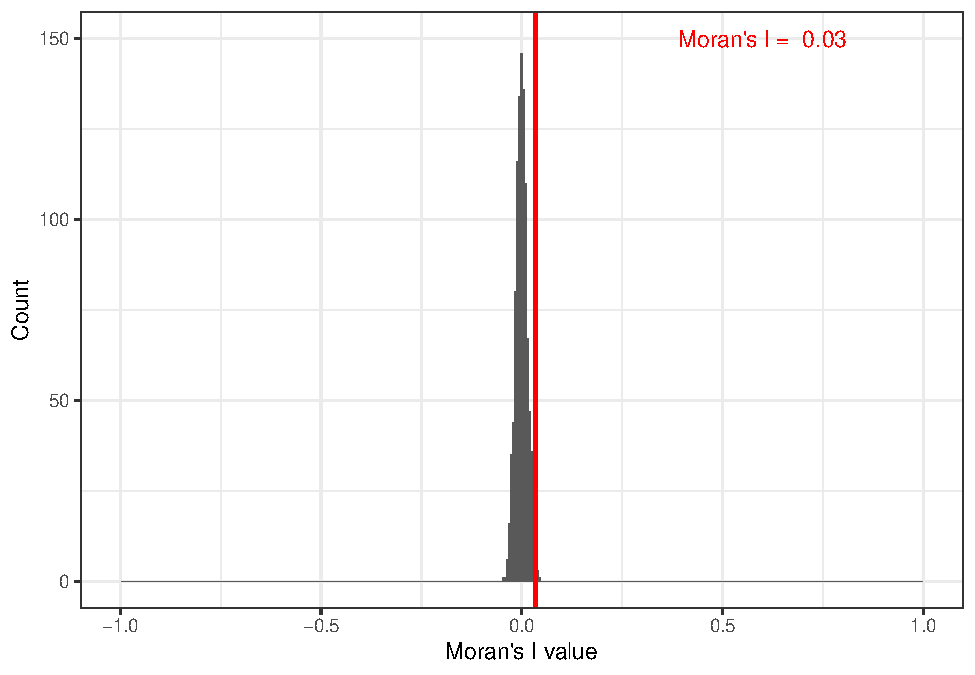
\includegraphics{HW3-LogisticRegression_files/figure-latex/unnamed-chunk-10-1.pdf}

We use the minimum distance approach to determine the threshold where
the distance from the top left hand corner to the ROC curve is lowest.
This approach helps determine the threshold where both the sensitivity
and specificity of the model predictions are minimized. The threshold
with the shortest distance from the ROC curve to the top left hand
corner is 0.06365151. At this threshold, the sensitivity is 0.66076459
and the specificity is 0.54524328.

\begin{verbatim}
##                   [,1]
## sensitivity 0.66076459
## specificity 0.54524328
## threshold   0.06365151
\end{verbatim}

We examine the AUC to measure the overall fit of our logistic model. As
discussed earlier, the closer the AUC value is to 1, the greater the
ability of the model to select a threshold which minimizes both
sensitivity and specificity. Our AUC value is 0.6398695 which indicates
a poor fit, based on the thresholds generally followed by statisticians.
The AUC value supports our previous conclusion that the ROC curve does
not have a good fit.

\begin{verbatim}
## [[1]]
## [1] 0.6398695
\end{verbatim}

\hypertarget{alternative-logistic-regression-model}{%
\subsubsection{Alternative Logistic Regression
Model}\label{alternative-logistic-regression-model}}

We present the results of an alternative logistic regression in which
the continuous variables (i.e: PCTBACHMOR and MEDHHINC) have been
removed and only the binary variables are included. We refer to this
alternative logistic regression as logistic regression 2. In logistic
regression 2, there are no major changes in the p-values of the
\(\beta\) coefficients. All binary variables except for CELL\_PHONE
continue to be statistically significant as the p-values are near zero,
and we can reject the null hypothesis that the \(\beta\) coefficient is
zero. Using the alternative logistic regression model results in small
changes to the \(\beta\) coefficients and odds ratio. For example, the
\(\beta\) coefficient for DRIVER1617 increases by 0.01 and the \(\beta\)
coefficient for CELL\_PHONE also increases by approximately 0.01.

\begin{verbatim}
## 
## Call:
## glm(formula = DRINKING_D ~ FATAL_OR_M + OVERTURNED + CELL_PHONE + 
##     SPEEDING + AGGRESSIVE + DRIVER1617 + DRIVER65PLUS, family = "binomial", 
##     data = data)
## 
## Coefficients:
##              Estimate Std. Error z value Pr(>|z|)    
## (Intercept)  -2.65190    0.02753 -96.324  < 2e-16 ***
## FATAL_OR_M    0.80932    0.08376   9.662  < 2e-16 ***
## OVERTURNED    0.93978    0.10903   8.619  < 2e-16 ***
## CELL_PHONE    0.03107    0.19777   0.157    0.875    
## SPEEDING      1.54032    0.08053  19.128  < 2e-16 ***
## AGGRESSIVE   -0.59365    0.04775 -12.433  < 2e-16 ***
## DRIVER1617   -1.27158    0.29311  -4.338 1.44e-05 ***
## DRIVER65PLUS -0.76646    0.09576  -8.004 1.21e-15 ***
## ---
## Signif. codes:  0 '***' 0.001 '**' 0.01 '*' 0.05 '.' 0.1 ' ' 1
## 
## (Dispersion parameter for binomial family taken to be 1)
## 
##     Null deviance: 19036  on 43363  degrees of freedom
## Residual deviance: 18344  on 43356  degrees of freedom
## AIC: 18360
## 
## Number of Fisher Scoring iterations: 6
\end{verbatim}

\begin{verbatim}
##                 Estimate Std. Error     z value     Pr(>|z|)         OR
## (Intercept)  -2.65189961 0.02753107 -96.3238683 0.000000e+00 0.07051713
## FATAL_OR_M    0.80931557 0.08376150   9.6621431 4.366327e-22 2.24636998
## OVERTURNED    0.93978420 0.10903433   8.6191585 6.744795e-18 2.55942903
## CELL_PHONE    0.03107367 0.19777088   0.1571195 8.751506e-01 1.03156149
## SPEEDING      1.54032033 0.08052787  19.1277908 1.482240e-81 4.66608472
## AGGRESSIVE   -0.59364687 0.04774781 -12.4329656 1.730916e-35 0.55230941
## DRIVER1617   -1.27157607 0.29310969  -4.3382260 1.436374e-05 0.28038936
## DRIVER65PLUS -0.76645727 0.09576440  -8.0035718 1.208612e-15 0.46465631
##                   2.5 %    97.5 %
## (Intercept)  0.06678642 0.0743978
## FATAL_OR_M   1.90112455 2.6404533
## OVERTURNED   2.05736015 3.1556897
## CELL_PHONE   0.68459779 1.4907150
## SPEEDING     3.97961862 5.4573472
## AGGRESSIVE   0.50268818 0.6061758
## DRIVER1617   0.14904734 0.4751771
## DRIVER65PLUS 0.38318289 0.5579332
\end{verbatim}

The table below shows the AIC for logistic regression 1. The model with
all nine predictors has an AIC value of 18359.63. The model with just
the seven binary predictors has an AIC value of 18360.47. Because the
logistic regression with all nine predictors has a lower AIC value we
can conclude that it has a better fit.

\begin{table}
\centering
\begin{tabular}[t]{l|r|r}
\hline
Regression & Number of Predictors & AIC\\
\hline
Logistic Regression 1 & 10 & 18359.63\\
\hline
Logistic Regression 2 & 8 & 18360.47\\
\hline
\end{tabular}
\end{table}

\hypertarget{discussion}{%
\subsection{Discussion}\label{discussion}}

Our analysis uses data from Pennsylvania Department of Transportation on
car crashes, and we use logistic regression models to model if a driver
will likely be drunk based on other variables. We include seven binary
variables, which are part of the original dataset from the Department of
Transportation dataset and two continuous variables which are derived
from census data (PCTBACHMOR, MEDHHINC).

Our model indicates that the variable which is the strongest predictors
of crashes involving drunk drivers is if the driver is speeding, which
has the highest odds ratio. Other variables which are predictive of
whether the driver will be drunk, based on our model, include if major
injuries or fatalities occurred in the accident, if the vehicle was
overturned, and if the driver was aggressive. The age of the driver
(i.e: if the driver is under eighteen or over 65) is also predictive,
but not as predictive as the other binary variables. Cell-phone use
during a crash is not predictive of one of the drivers in an accident
drunk driving.

The results are unsurprising, and variables we most suspected to be
associated with drunk driving were significant. The odds ratios for a
major injury or fatality occuring in an accident, a car being overturned
and a driver speeding in an accident are all greater than one. Thus,
these variables have a higher likelihood of occurring during an accident
if the driver is drunk. One surprising and unexpected finding is that
the odds ratio for aggressive driving is less than one, indicating that
drivers who are drunk during an accident are less likely to also be
driving aggressively during an accident.

While the proportion of crashes that involve drunk drivers comprise only
5\% of the total incidents of crashes in our data set, there are nearly
2,500 crashes involving drunk drivers. Given this high number of cases
in the less likely of our two outcomes, logistic regression appears to
be a viable method for analyzing our data due to a large enough sample
size of rare events. However, we could still consider using the
penalized likelihood methodology proposed by Paul Allison when
discussing rare events to account for the small proportion of drunk
driving accidents in the data.

Some of the limitations of the analysis include the overall poor fit of
the model. The AUC value is indicative of a poor model. Adding
predictors through feature engineering and new data could help improve
the predictive power of the model and increase the AUC value.

Additionally, the usage of Pearson's correlation to check for
multicollinearity has limitations when working with binary data as it is
typically used for continuous data. In order to strengthen the
conclusion that multicollinearity is not present, other
multicollinearity tests such as the Variance Inflation Factor could be
examined.

\end{document}
